\section{Application to vacuum spectra}
\label{sec:results_vacuum}

Now we move to present the application of the strategy presented in the previous
section to the parametrisation of the ZLP spectra taken in vacuum.
%
Applying our model to this case has a two-fold motivation.
%
First of all, we aim to demonstrate that our model is flexible enough to effectively reproduce the
input EELS measurements for a range of variations of the operation parameters of the microscope.
%
Second, it will allow us to provide a calibration prediction for the case of the in-sample measurements.
%
Such calibration is necessary since, as explained in Sect.~\ref{sec:training}, some of the model
hyper-parameters are determined by the comparison of the intensity derivatives
between spectra taken in vacuum and those in sample.

In Table~\ref{table:vacuumdata} we collect the main properties of the EELS spectra acquired in vacuum to train the neural
    network model.  For each set of spectra, we indicate the exposure time $t_{\rm exp}$, the beam energy
    $E_b$, the number of spectra $N_{\rm sp}$ corresponding to these operation conditions, the number $N_{\rm dat}$ of
    bins in each spectrum, the range in electron energy loss $\Delta E$,
    and the average full width at half maximum (FWHM)
    evaluated over the $N_{\rm sp}$ spectra with the corresponding variance.
    %
    The data sets were recorded with a Titan TEM equipped with a Schottky field emitter.
    %
    Since we are interested in the low-loss region, $\Delta E_{\rm max}$ does not need
    to be too large, and in any case the large $|\Delta E|$ behaviour of the model is fixed
    by the constraint implemented by means of Eq.~(\ref{eq:chi2modified}).
    %
    The energy resolution of these spectra, quantified by the value of the FWHM, ranges
    from 3 eV to 25 eV depending on the specific operation conditions of the microscope.
    %
    A total of 81920 independent measurements will be thus used for the ZLP model
    training on the vacuum spectra.
    %
    As we show below, one of the advantages of our model is that it can extrapolate the ZLP predictions
    for other operation conditions of the microscope beyond those used for the training.

%%%%%%%%%%%%%%%%%%%%%%%%%%%%%%%%%%%%%%%%%%%%%%%%%%%%%%%%%%%%%%%%%%%%%%%%%%%%%%%%%%%%%%%%%%%%%
%%%%%%%%%%%%%%%%%%%%%%%%%%%%%%%%%%%%%%%%%%%%%%%%%%%%%%%%%%%%%%%%%%%%%%%%%%%%%%%%%%%%%%%%%%%%%
\begin{table}[t]
  \begin{center}
            \renewcommand{\arraystretch}{1.50}
  \begin{tabular}{@{}ccccccccc}
\br
Set & $t_{\rm exp}$ {(}ms{)} & $E_{\rm b}$ {(}keV{)} & $N_{\rm sp}$ & $N_{\rm dat}$ & $\Delta E_{\rm min}$~(eV)  & $\Delta E_{\rm max}$~(eV)  & FWHM~(eV)  \\ 
\mr
1        & 100                 & 200                  & 15          & 2048               & -0.96              & 8.51     & $0.025\pm$         \\
2        & 100                 & 60                   & 7           & 2048               & -0.54              & 5.59    & $ 0.022\pm$         \\
3        & 10                  & 200                  & 12          & 2048               & -0.18              & 2.97      & $0.003\pm$         \\
4        & 10                  & 60                   & 6           & 2048               & -0.40              & 4.78       & $0.017\pm$         \\ 
\br
  \end{tabular}
    \end{center}
  \caption{\small Summary of the main properties of the EELS spectra acquired in vacuum to train the neural
    network model.  For each set of spectra, we indicate the exposure time $t_{\rm exp}$, the beam energy
    $E_b$, the number of spectra $N_{\rm sp}$ corresponding to these operation conditions, the number $N_{\rm dat}$ of
    bins in each spectrum, the range in electron energy loss $\Delta E$,
    and the average FWHM evaluated over the $N_{\rm sp}$ spectra with the corresponding variance.
  }
   \label{table:vacuumdata}
\end{table}
%%%%%%%%%%%%%%%%%%%%%%%%%%%%%%%%%%%%%%%%%%%%%%%%%%%%%%%%%%%%%%%%%%%%%%%%%%%%%%%%%%%%%%%%%%%%%%%%%5
%%%%%%%%%%%%%%%%%%%%%%%%%%%%%%%%%%%%%%%%%%%%%%%%%%%%%%%%%%%%%%%%%%%%%%%%%%%%%%%%%%%%%%%%%%%%%

Following the strategy presented in Sect.~\ref{sec:methodology}, first of all we combine the $N_{\rm sp}$ spectra
corresponding to each of the four sets of operation conditions and determine the statistical uncertainty
associated to each energy loss bin by means of Eq.~(\ref{eq:sigmaiexp}).
%
We use this information to generate a sample of $N_{\rm rep}=500$ Monte Carlo replicas of the input data listed
in Table~\ref{table:vacuumdata} and train an individual neural network model to each of these replicas.
%
The end result of the procedure is a set of model replicas, $I_{\rm ZLP}^{\rm (mod)(k)}(\Delta E, E_{b},t_{\rm exp})$,
which can be used to provide a prediction for the intensity of the ZLP
for arbitrary values of $\Delta E$,  $E_{b}$, and $t_{\rm exp}$.
%
This sample provides a representation of the probability density in the space of $I_{\rm ZLP}$ models, from which
statistical estimators such as averages, variances, and correlations can be evaluated by means of
the standard MC expressions, namely
\be
\label{eq:average}
\la I_{\rm ZLP}^{\rm (mod)}(\Delta E, E_{b},t_{\rm exp}) \ra = \frac{1}{N_{\rm rep}}\sum_{k=1}^{N_{\rm rep}}
I_{\rm ZLP}^{\rm (mod)(k)}(\Delta E, E_{b},t_{\rm exp}) \, ,
\ee
\be
\label{eq:standarddev}
\sigma_{I_{\rm ZLP}}^{\rm (mod)}(\Delta E, E_{b},t_{\rm exp})  = \lp \frac{1}{N_{\rm rep}-1} \sum_{k=1}^{N_{\rm rep}}
\lp  I_{\rm ZLP}^{\rm (mod)(k)}  - \la I_{\rm ZLP}^{\rm (mod)}  \ra   \rp \rp^{1/2} \, ,
\ee
\be
\rho \lp \{z_1\},\{z_2\}\rp = \frac{ \la I_{\rm ZLP}^{\rm (mod)}( \{z_1\} ) I_{\rm ZLP}^{\rm (mod)}( \{z_2\} ) \ra
- \la I_{\rm ZLP}^{\rm (mod)}( \{z_1\} )\ra \la I_{\rm ZLP}^{\rm (mod)}( \{z_2\} ) \ra}{\sigma_{I_{\rm ZLP}}^{\rm (mod)}( \{z_1\} )\sigma_{I_{\rm ZLP}}^{\rm (mod)}( \{z_2\} )}
\ee
where as in the previous section $\{z_l\}$ denotes a possible set of input variables for the model.
We now discuss some of features of this ZLP vacuum model.

\paragraph{Fit quality.}
%
To begin with we would like to quantify the overall fit quality of the model and demonstrate that it is flexible enough
to describe all the available input datasets.
%
In Table~\ref{table:chi2summary} we indicate the values of the final $\chi^2$ per data point,
    Eq.~(\ref{eq:chi2_final}), as well as the average values of the error Eq.~(\ref{eq:chi2})
    over the training and validation subsets, for each of the four sets of spectra listed in
    Table~\ref{table:vacuumdata} as well as for the total dataset.
    %
    We recall that for a satisfactory training one expects $\chi^2 \simeq 1$
    and $\la E_{\rm tr}\ra \simeq \la E_{\rm val}\ra \simeq 2 $~\cite{Forte:2002fg}.
    %
    From the results of this table we can see that ....

%%%%%%%%%%%%%%%%%%%%%%%%%%%%%%%%%%%%%%%%%%%%%%%%%%%%%%%%%%%%%%%%%%%%%%%%%%%%%%%%%%%%%%%%%%%%%
%%%%%%%%%%%%%%%%%%%%%%%%%%%%%%%%%%%%%%%%%%%%%%%%%%%%%%%%%%%%%%%%%%%%%%%%%%%%%%%%%%%%%%%%%%%%%
\begin{table}[t]
  \begin{center}
            \renewcommand{\arraystretch}{1.35}
  \begin{tabular}{@{}cccc}
\br
Set & $\chi^2$  &  $\la E_{\rm tr}\ra$   &  $\la E_{\rm val}\ra$ \\
\mr
1        &                 &                  &    \\
2        &                  &                   &      \\
3        &                   &                   &     \\
4        &                   &                    &      \\
\mr
Total    &                     &                      &      \\
\br
  \end{tabular}
    \end{center}
  \caption{\small The values of the final $\chi^2$ per data point,
    Eq.~(\ref{eq:chi2_final}), as well as the average values of the error Eq.~(\ref{eq:chi2})
    over the training and validation subsets, for each of the four sets of spectra listed in
    Table~\ref{table:vacuumdata} as well as for the total dataset.
  }
   \label{table:chi2summary}
\end{table}
%%%%%%%%%%%%%%%%%%%%%%%%%%%%%%%%%%%%%%%%%%%%%%%%%%%%%%%%%%%%%%%%%%%%%%%%%%%%%%%%%%%%%%%%%%%%%%%%%5
%%%%%%%%%%%%%%%%%%%%%%%%%%%%%%%%%%%%%%%%%%%%%%%%%%%%%%%%%%%%%%%%%%%%%%%%%%%%%%%%%%%%%%%%%%%%%

\paragraph{Dependence on the electron energy loss $\Delta E$.}
%
Having demonstrated that our neural network model provides a satisfactory description
of all the input EEL spectra, we now present predictions for specific input parameters.
%
First of all, we investigate the dependence of the results as a function of the
electron energy loss $\Delta E$.
%
In the left panel of Fig.~\ref{fig:EELS_vacuum_DeltaE} we show the central value and 68\% confidence level uncertainty band of the ZLP model as a function
of $\Delta E$,
evaluated using Eqns.~(\ref{eq:average}) and~(\ref{eq:standarddev}), for $t_{\rm exp}=100$ ms
and $E_{b}=60$ and 200 keV.
%
The inset displays the relative model uncertainty as a function of $\Delta E$.
%
We can observe the differences in the ZLP predictions as the electron beam energy $E_b$ is varied.
%
The relative uncertainties in the model turn out to be around 20\%, more or less independent
of the electron energy loss.

It is interesting to assess how the model results are modified once a subset of the data points
are excluded from the fit.
%
As illustrated in Fig.~\ref{fig:EELS_toy}, when training the model on sample spectra, a region
with $\Delta E_I \le \Delta E \le \Delta E_{II}$ will be removed from the training dataset to avoid the
contamination from the inelastic contributions.
%
To emulate the effects of such cut, in the right panel of Fig.~\ref{fig:EELS_vacuum_DeltaE} we
display the same comparison of the left one but now
for the case in which the input data bins with $\Delta E \ge 50$ meV are excluded from the fit.
%
In this way we test the extrapolation properties of the model between the data region ($\Delta E < 50$ meV)
and the region where $I_{\rm ZLP}(\Delta E)$ is forced to vanish.
%
If we compare the relative model uncertainties between the two cases, one can observe the expected
increase in the errors where a fraction of the input data has been cut away.
%
The same qualitative behaviour appears for the two values of $E_b$ considered here.
%
The comparisons of Fig.~\ref{fig:EELS_vacuum_DeltaE} indicate that our model uncertainties
indeed translate in an appropriate way the information contained in the training dataset -- note that
this would not be the case had one one a simple functional fit to model the ZLP.

%%%%%%%%%%%%%%%%%%%%%%%%%%%%%%%%%%%%%%%%%%%%%%%%%%%%%%%%%%%%%%%%%%%%%%%%%%%%%%%%%%%%%%%%%%%%%%%%%%%%%%%%%%%%
\begin{figure}[h]
    \centering
    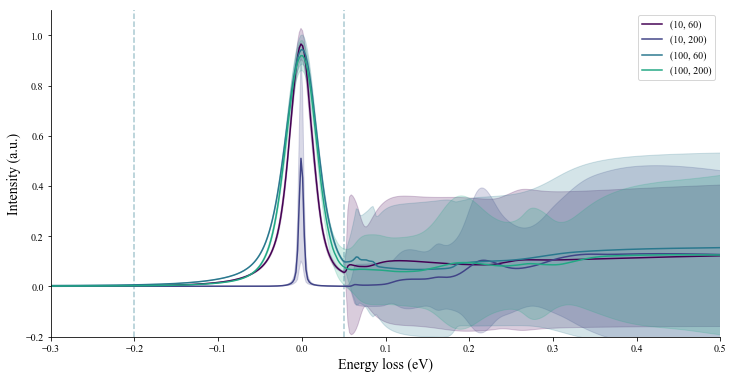
\includegraphics[width=120mm]{plots/extrapolate_energyloss.png}
    \caption{Left panel: the central value and 68\% confidence level uncertainty band of the ZLP model as a function
      of $\Delta E$,
      evaluated using Eqns.~(\ref{eq:average}) and~(\ref{eq:standarddev}), for $t_{\rm exp}=100$ ms
      and $E_{b}=60$ and 200 keV.
      %
      The inset displays the relative model uncertainty as a function of $\Delta E$.
      %
      Right panel: same now for the case where the input data with $\Delta E \ge 50$ meV is excluded from the fit.
      {\bf  ToDo}}
    \label{fig:EELS_vacuum_DeltaE}
\end{figure}
%%%%%%%%%%%%%%%%%%%%%%%%%%%%%%%%%%%%%%%%%%%%%%%%%%%%%%%%%%%%%%%%%%%%%%%%%%%%%%%%%%%%%%%%%%%%%%%%%%%%%%%%%%%%%%%%%%%

\paragraph{Dependence on the beam energy $E_b$.}
%
As indicated in Table~\ref{table:vacuumdata}, the training dataset contains
spectra taken at two values of the electron beam energy, $E_b=60$ keV and 300 keV.
%
Fig.~\ref{fig:extrapolbeam} displays  model predictions for the FWHM of the zero loss peak
      (and its corresponding uncertainty) as a function of the beam energy $E_b$
      for two values of the exposure time, $t_{\rm exp}=10$ ns and 100 ms.
      %
      The vertical dashed lines indicate the values of $E_b$ for which training data is available.
      %
      This comparison illustrates how the model uncertainty vary in the data region
      (near $E_b=60$ keV and 200 keV), the interpolation region (for $E_b$ between 60 and 200 keV),
      and the extrapolation regions (for $E_b$ below 60 keV and above 200 keV).
      
%%%%%%%%%%%%%%%%%%%%%%%%%%%%%%%%%%%%%%%%%%%%%%%%%%%%%%%%%%%%%%%%%%%%%%%%%%%%%%%%%%%%%%%
\begin{figure}[t]
    \centering
    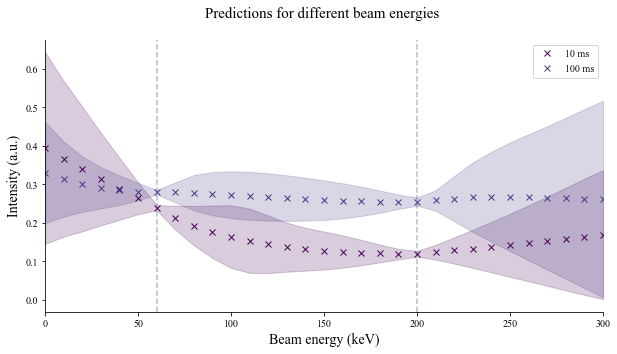
\includegraphics[width=130mm]{plots/Extrapolate_beamenergy.png}
    \caption{The model predictions for the FWHM of the zero loss peak
      (and its corresponding uncertainty) as a function of the beam energy $E_b$
      for two values of the exposure time, $t_{\rm exp}=10$ ns and 100 ms.
      %
      The vertical dashed lines indicate the values of $E_b$ for which training data is available,
      namely $E_b=60$ keV and 200 keV. {\bf ToDo}
    }
    \label{fig:extrapolbeam}
\end{figure}
%%%%%%%%%%%%%%%%%%%%%%%%%%%%%%%%%%%%%%%%%%%%%%%%%%%%%%%%%%%%%%%%%%%%%%%%%%%%%%%%%%%%%%%%%%%%

For this comparison one can observe that as expected the uncertainty in the  prediction for FWHM
of the ZLP is the smallest close to the values of $E_b$ for which one has training data.
%
The uncertainties increase but only in a moderate way in in the interpolation region, indicating that
the model can be reliable applied to predict the features of the ZLP other values of the electron
energy beam (assuming that all other operation conditions of the microscope are unchanged).
%
The errors increase rapidly in the extrapolation region, which is a characteristic feature of
these neural network models.
%
Indeed, as soon as the model departs from the data region there exist a very large
number of different functional form models for $I_{\rm ZLP}(\Delta E)$ that can describe equally well
the training dataset, and hence a blow up of the extrapolation uncertainties is generically expected.

\paragraph{Dependence on the exposure time $t_{\rm exp}$.}
%
The network was trained on data with exposure times of $10$ and $100$ ms, so interpolation and extrapolation is possible. Similar to the predictions for varying beam energy, also for exposure time the uncertainties grow bigger as the value deviates more from the training inputs.
%
In Fig.~\ref{fig:extrapotime} we display a similar comparison as in
as Fig.~\ref{fig:extrapolbeam} now for the model
      predictions as a function of the exposure time $t_{\rm exp}$
for two values of the electron beam energy, $E_b=$ 60 keV and 200 keV.

%%%%%%%%%%%%%%%%%%%%%%%%%%%%%%%%%%%%%%%%%%%%%%%%%%%%
\begin{figure}[t]
  \centering
    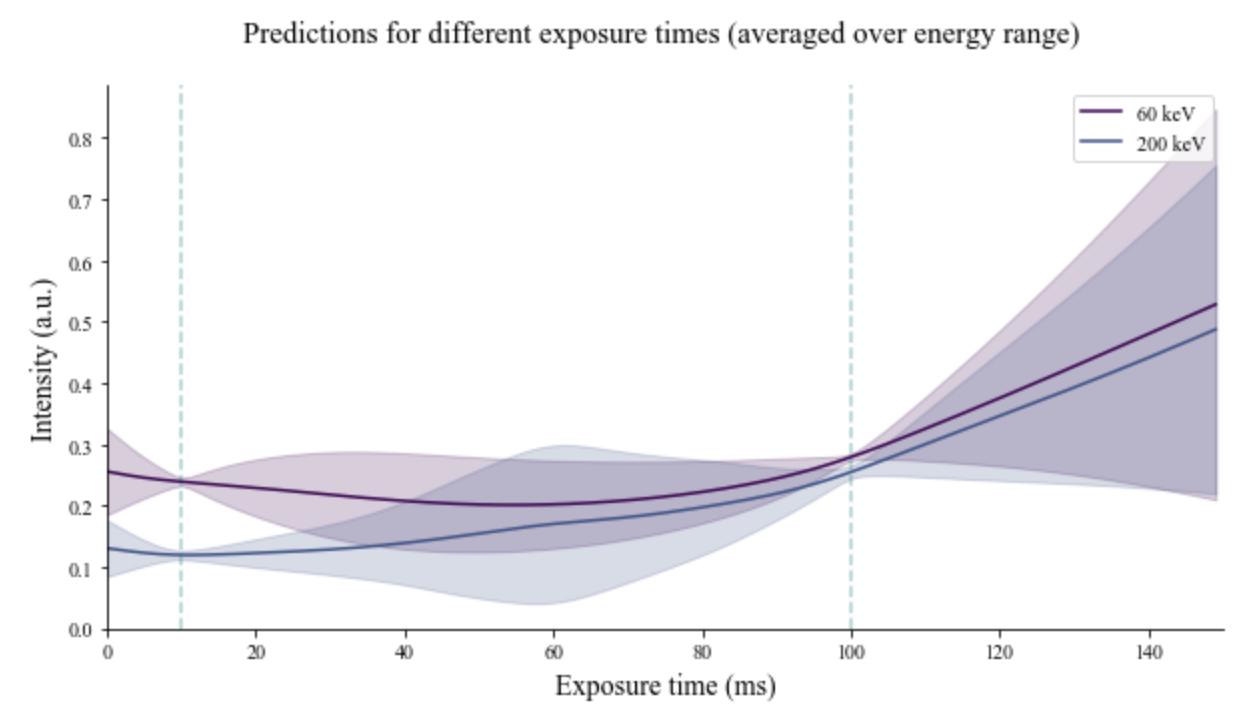
\includegraphics[width=120mm]{plots/Extrapolate_exposuretime.png}
    \caption{Same as Fig.~\ref{fig:extrapolbeam} now displaying the model
      predictions as a function of the exposure time $t_{\rm exp}$
for two values of the electron beam energy, $E_b=$ 60 keV and 200 keV.
      {\bf ToDo}}
    \label{fig:extrapotime}
\end{figure}
%%%%%%%%%%%%%%%%%%%%%%%%%%%%%%%%%%%%%%%%%%%%%%%%
